\documentclass{sigchi}

% Use this command to override the default ACM copyright statement (e.g. for preprints). 
% Consult the conference website for the camera-ready copyright statement.


%% EXAMPLE BEGIN -- HOW TO OVERRIDE THE DEFAULT COPYRIGHT STRIP -- (July 22, 2013 - Paul Baumann)
% \toappear{Permission to make digital or hard copies of all or part of this work for personal or classroom use is 	granted without fee provided that copies are not made or distributed for profit or commercial advantage and that copies bear this notice and the full citation on the first page. Copyrights for components of this work owned by others than ACM must be honored. Abstracting with credit is permitted. To copy otherwise, or republish, to post on servers or to redistribute to lists, requires prior specific permission and/or a fee. Request permissions from permissions@acm.org. \\
% {\emph{CHI'14}}, April 26--May 1, 2014, Toronto, Canada. \\
% Copyright \copyright~2014 ACM ISBN/14/04...\$15.00. \\
% DOI string from ACM form confirmation}
%% EXAMPLE END -- HOW TO OVERRIDE THE DEFAULT COPYRIGHT STRIP -- (July 22, 2013 - Paul Baumann)


% Arabic page numbers for submission. 
% Remove this line to eliminate page numbers for the camera ready copy
% \pagenumbering{arabic}


% Load basic packages
\usepackage{balance}  % to better equalize the last page
\usepackage{graphics} % for EPS, load graphicx instead
\usepackage{times}    % comment if you want LaTeX's default font
\usepackage{url}      % llt: nicely formatted URLs

% llt: Define a global style for URLs, rather that the default one
\makeatletter
\def\url@leostyle{%
  \@ifundefined{selectfont}{\def\UrlFont{\sf}}{\def\UrlFont{\small\bf\ttfamily}}}
\makeatother
\urlstyle{leo}


% To make various LaTeX processors do the right thing with page size.
\def\pprw{8.5in}
\def\pprh{11in}
\special{papersize=\pprw,\pprh}
\setlength{\paperwidth}{\pprw}
\setlength{\paperheight}{\pprh}
\setlength{\pdfpagewidth}{\pprw}
\setlength{\pdfpageheight}{\pprh}

% Make sure hyperref comes last of your loaded packages, 
% to give it a fighting chance of not being over-written, 
% since its job is to redefine many LaTeX commands.
\usepackage[pdftex]{hyperref}
\hypersetup{
pdftitle={},
pdfauthor={LaTeX},
pdfkeywords={SIGCHI, proceedings, archival format},
bookmarksnumbered,
pdfstartview={FitH},
colorlinks,
citecolor=black,
filecolor=black,
linkcolor=black,
urlcolor=black,
breaklinks=true,
}

% create a shortcut to typeset table headings
\newcommand\tabhead[1]{\small\textbf{#1}}
\newcommand{\putat}[3]{\begin{picture}(0,0)(0,0)\put(#1,#2){#3}\end{picture}}

% End of preamble. Here it comes the document.
\begin{document}

\title{Sovereignty of the people: \\introducing app-usage and trend filters based on actual popularity and usage rather than recommendations}

\numberofauthors{3}
\author{
  \alignauthor 1st Author Name\\
    \affaddr{Affiliation}\\
    \affaddr{Address}\\
    \email{e-mail address}\\
    \affaddr{Optional phone number}
  \alignauthor 2nd Author Name\\
    \affaddr{Affiliation}\\
    \affaddr{Address}\\
    \email{e-mail address}\\
    \affaddr{Optional phone number}    
  \alignauthor 3rd Author Name\\
    \affaddr{Affiliation}\\
    \affaddr{Address}\\
    \email{e-mail address}\\
    \affaddr{Optional phone number}
}

\maketitle
\putat{310}{130}{
\includegraphics[height=1cm]{Figures/appstorePeople03.png}}
\begin{abstract}
In this paper we describe the formatting requirements for
SIGCHI Conference Proceedings, and this sample file
offers recommendations on writing for the worldwide
SIGCHI readership. Please review this document even if
you have submitted to SIGCHI conferences before, some
format details have changed relative to previous years.

\end{abstract}

\keywords{
	Guides; instructions; author's kit; conference publications;
	keywords should be separated by a semi-colon. \newline
	\textcolor{red}{Optional section to be included in your final version, 
  but strongly encouraged.}
}

\category{H.5.m.}{Information Interfaces and Presentation (e.g. HCI)}{Miscellaneous}

See: \url{http://www.acm.org/about/class/1998/}
for more information and the full list of ACM classifiers
and descriptors. \newline
\textcolor{red}{Optional section to be included in your final version, 
but strongly encouraged. On the submission page only the classifiers’ 
letter-number combination will need to be entered.}

\section{Introduction}

% 1000 ??? apps but which is the really good one?
% -- paula: Find the app that I want for my category
% -- me: From these, identify the flops and topps.
% 
% -- Also: Identify the real popular apps and trends not from absolute usage but relative usage 
% -- And: Be among the first to identify a trend and jump off before it is over.


% http://www.statista.com/statistics/266210/number-of-available-applications-in-the-google-play-store/
% http://www.statista.com/statistics/276623/number-of-apps-available-in-leading-app-stores/
With continuing popularity of current smartphone operating systems, the number of available apps in the respective app stores continues to grow rapidly.
The google play store currently features more than 1.4 million apps and Apple's IOS app store more than 1.3 million apps. 
Follow-ups are the windows playstore ($>$300.000), Amazon appstore ($>240.000$) and BlackBerry world ($>130.000$)\footnote{http://www.statista.com/statistics/276623/number-of-apps-available-in-leading-app-stores/}.

It has become easy to find an app for virtually any possible category but challenging to identify good and reliable apps from this overwhelming assortment. 
Often, this tedious process might involve installing multiple apps and testing each of them individually. 
Although users are typically supported by a recommendation system in which apps can be rated on, such systems favour apps with a bigger crowd of users such as corporation-developed apps or older and therefore better known apps.
For instance, an app which is popular and frequently used in a small community of users might have low chance to be discovered by a greater public due to less ratings. 
Absolute user number wins over relative high satisfaction of a smaller crowd of app-users.
Paradoxically, offensively annoying users to submit recommendations is a superior strategy to just satisfying users with a superb app.  

Furthermore, the system can be to some extent subject to fraud. 
And, most importantly, since they are based on historical data, recommendations might not reflect the actual usage patterns as well as current popularity and trends.

We propose the use of an app-usage filter which shows actual relative popularity of apps based on their daily usage, indicates trends regardless of absolute volume and identifies app-lifecycles. 
Lifecycles are, for instance, flops, dead applications, trendy apps quickly gaining users as well as apps of continouous high popularity. 

We exploit the Carat data \textbf{\cite{???}} collected from \textbf{???} phones over a period of \textbf{???} months (\textbf{???} till \textbf{???}) to demonstrate our approach.
Based on this data, we cluster app-usage time series with similar patterns together in order to identify typical app life-cycles.

From these lifecycle-templates we are then able with alignment matching methods to identify for new apps at which stage in the lifecycle they are currently.

\section{Related Work}


\section{Overview}
Overall, our system consists of several modules to process the app-time-series data. 
First, we extract from the CARAT usage statistics (count of installations of a specific app on a daily basis) the usage frequency for individual apps.
This time series is potentially discontinuous and absolute numbers vary greatly among distinct apps.

Therefore, as a next step, these time sereis are then normalised to relative usage counts between 0 and 1, where 1 corresponds to the maximum usage count. 
In addition, missing values for intermediate days are interpolated so taht each time series has a valid value on each day.

These time series are then clustered for similar time-series patterns.
The idea behind this is that an app undergoes an app-lifecycle and that it might be possible to represent this lifecycle with these usage patterns.
We aim to group alll app with similar lifecycles together.

For this, time-series are first aligned at their peak before clustering them with k-means clustering approach.
Features for the k-means are the variance of the time series, the area under the curve and the location of the peak relateive to the time-series length.

From each cluster, a consensus-lifecycle as a representative is generated by calculating for each respective day the mean from all time series in that cluster. 

For a time-series of a new app, we are then able to identify the consensus-lifecycle to which it is most similar and where in that lifecycle it currently is by applying alignment methods as described in section~\ref{sectionAligment}.



Description of the system (schematic view)
\begin{itemize}
 \item normalize
 \item shift and interpolate
 \item cluster (k-means + features)
 \item Consensus
 \item Alignment (see ISWC note)
\end{itemize}
\subsection{Normalisation of Timeseries to make them comparable}
normalise, shift, interpolate
\subsection{Clustering timeseries}
k-means and features
\subsection{Compute consensus timeseries}
explain the approach
\subsection{Alignment to find trend-state}\label{sectionAlignment}
\textbf{explain alignment method -- revise below text}

In the algorithm, two strings are compared for the best approximative pattern among them, as depicted in figure~\ref{figurePatternMatching}.
\begin{figure}
      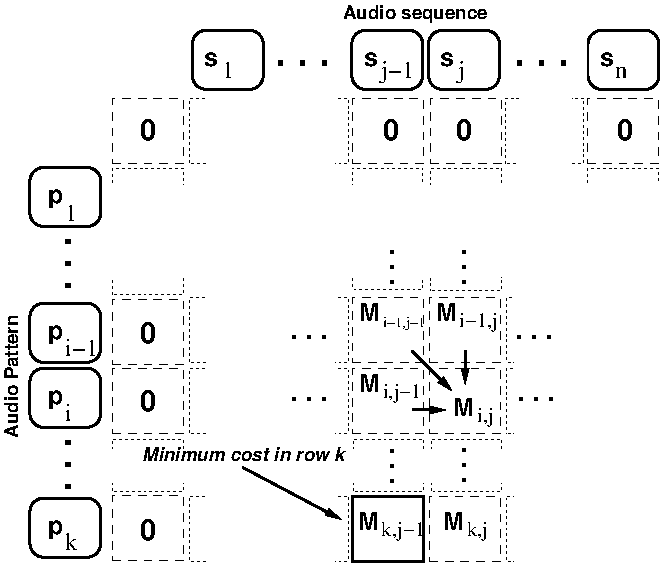
\includegraphics[width=8cm, height=4.5cm]{AlignmentScheme_120130_v7_STS.pdf}
     \caption{Schematic illustration of the Smith-Waterman pattern matching}
     \label{figurePatternMatching}
\end{figure}
The figure illustrates the operation to find a sub-sequence similar to a pattern $p=p_1\dots p_k$ in a longer sequence $s=s_1\dots s_n$.
The matrix is filled from left to right and from top to bottom.
Each matrix entry $M_{ij}$ contains the minimum cost to align $p_1\dots p_i$ with $s_1\dots s_j$.
It is obtained iteratively from the cost of the cells $M_{i-1,j-1},M_{i-1,j},M_{i,j-1}$ by choosing the minimum cost for an extension of any of these three alignments (extension of both strings, extension of only the first string or extension of only the second string).
The first row is initialised with $0$ to allow the pattern to start at any position within $s$.
The careful choice of the gap-penalty $g$ is crucial for the approach to produce good matching results.
The best matching string is obtained by backtracking the smallest entry in the last row.

Since the matching is approximative, we will always find a best matching position even though the absolute similarity of this very position might not be high.
we exploit this property to be able to resign from any information transmitted among devices on the actual recorded audio.
In particular, we utilize a predefined, characteristic pattern on both devices.
since the pattern is known in advance, no information need to be transmitted.
The downside to this implementation is, of course, that the pattern utilised might be very different from the actual audio recorded.
However, since the Smith-Waterman algorithm always computes a best matching, we can speculate that this best matching is found at similar positions in the audio recordings, provided that the data has significant similarity.
The best matching, although it might not be a good matching in absolute terms, is likely to be found at a similar position in the recorded audio of the remote devices.

The specific pattern used for matching is extracted randomly from consecutive samples of an arbitrary audio sequence. 
In our experiments, its length is 100 samples. Longer patterns increase running time of the algorithm without improving the accuracy of the matching. 
Due to the fact that our sampling rate is 44100Hz, a 100-sample pattern is equivalent to a 0.003-second audio chunk. 

The pattern $p$ is matched in the first part of each audio file $s$, which is $100000$ samples long. 
The matching score of $p$ and a local part $l$ of $s$ is the difference between amplitude values in $p$ and $l$. 
The less the score, the more similar $p$ and $l$ are.
We maintain a matrix to store the scores  and another for tracing. 
Backtracking starts at the lowest scoring matrix cell. 
According to our experiments, the gap penalty that can yield an acceptable matching is $150$. 
After finding the matching position, we can eliminate all samples preceding this position and generate the audio fingerprint from the remaining ones.


\section{Paulas method}

\section{results}
\begin{itemize}
\item top 102 apps
\item 4 clusters
\item show the four clusters (timeseries)
\item and also show the consensus TS for each
\end{itemize}


\section{conclusion}

\section{Acknowledgments}

% We thank CHI, PDC and CSCW volunteers, and all publications support
% and staff, who wrote and provided helpful comments on previous
% versions of this document.  Some of the references cited in this paper
% are included for illustrative purposes only.  \textbf{Don't forget
% to acknowledge funding sources as well}, so you don't wind up
% having to correct it later.

% Balancing columns in a ref list is a bit of a pain because you
% either use a hack like flushend or balance, or manually insert
% a column break.  http://www.tex.ac.uk/cgi-bin/texfaq2html?label=balance
% multicols doesn't work because we're already in two-column mode,
% and flushend isn't awesome, so I choose balance.  See this
% for more info: http://cs.brown.edu/system/software/latex/doc/balance.pdf
%
% Note that in a perfect world balance wants to be in the first
% column of the last page.
%
% If balance doesn't work for you, you can remove that and
% hard-code a column break into the bbl file right before you
% submit:
%
% http://stackoverflow.com/questions/2149854/how-to-manually-equalize-columns-
% in-an-ieee-paper-if-using-bibtex
%
% Or, just remove \balance and give up on balancing the last page.
%
\balance

% \section{References format}
% References must be the same font size as other body text.
% % REFERENCES FORMAT
% % References must be the same font size as other body text.

\bibliographystyle{acm-sigchi}
\bibliography{sample}
\end{document}
